\documentclass[12pt,a4paper,bibliography=totocnumbered,listof=totocnumbered]{scrartcl}
\usepackage[ngerman]{babel}
\usepackage[utf8]{inputenc}
\usepackage{amsmath}
\usepackage{amsfonts}
\usepackage{amssymb}
\usepackage{graphicx}
\usepackage{fancyhdr}
\usepackage{tabularx}
\usepackage{geometry}
\usepackage{setspace}
\usepackage[right]{eurosym}
\usepackage[printonlyused]{acronym}
\usepackage{subfig}
\usepackage{floatflt}
\usepackage[usenames,dvipsnames]{color}
\usepackage{colortbl}
\usepackage{paralist}
\usepackage{array}
\usepackage{titlesec}
\usepackage{parskip}
\usepackage[right]{eurosym}

\usepackage[subfigure,titles]{tocloft}
\usepackage[pdfpagelabels=true]{hyperref}

\usepackage{listings}
\lstset{basicstyle=\footnotesize, captionpos=b, breaklines=true, showstringspaces=false, tabsize=2, frame=lines, numbers=left, numberstyle=\tiny, xleftmargin=2em, framexleftmargin=2em}
\makeatletter
\def\l@lstlisting#1#2{\@dottedtocline{1}{0em}{1em}{\hspace{1,5em} Lst. #1}{#2}}
\makeatother

\geometry{a4paper, top=27mm, left=30mm, right=20mm, bottom=35mm, headsep=10mm, footskip=12mm}

\hypersetup{unicode=false, pdftoolbar=true, pdfmenubar=true, pdffitwindow=false, pdfstartview={FitH},
	pdftitle={Fallstudie GIT},
	pdfauthor={Vedad Hamamdzic},
	pdfsubject={Abschlussarbeit},
	pdfcreator={\LaTeX\ with package \flqq hyperref\frqq},
	pdfproducer={pdfTeX \the\pdftexversion.\pdftexrevision},
	pdfkeywords={Ausarbeitung},
	pdfnewwindow=true,
	colorlinks=true,linkcolor=black,citecolor=black,filecolor=magenta,urlcolor=black}
\pdfinfo{/CreationDate (D:20110620133321)}

\begin{document}

\titlespacing{\section}{0pt}{12pt plus 4pt minus 2pt}{-6pt plus 2pt minus 2pt}

% Kopf- und Fusszeile
\renewcommand{\sectionmark}[1]{\markright{#1}}
\renewcommand{\leftmark}{\rightmark}
\pagestyle{fancy}
\lhead{}
\chead{}
\rhead{\thesection\space\contentsname}
\lfoot{Fallstudie Entwicklungswerkzeuge: GIT\newline}
\cfoot{}
\rfoot{\ \linebreak Seite \thepage}
\renewcommand{\headrulewidth}{0.4pt}
\renewcommand{\footrulewidth}{0.4pt}

% Vorspann
\renewcommand{\thesection}{\Roman{section}}
\renewcommand{\theHsection}{\Roman{section}}
\pagenumbering{Roman}

% ----------------------------------------------------------------------------------------------------------
% Titelseite
% ----------------------------------------------------------------------------------------------------------
\thispagestyle{empty}
\begin{center}
	
\includegraphics[scale=1]{Bilder/hs_os.png}\\
	\vspace*{2cm}
	\Large
	\textbf{Fallstudie Entwicklungswerkzeuge}\\
	\textbf{}\\
	\vspace*{2cm}
	\Huge
	\textbf{Ausarbeitung}\\
	\vspace*{0.5cm}
	\large
	über das Thema\\
	\vspace*{1cm}
	\textbf{GIT Versionsverwaltungssystem}\\
	\vspace*{2cm}
	
	\vfill
	\normalsize
	\newcolumntype{x}[1]{>{\raggedleft\arraybackslash\hspace{0pt}}p{#1}}
	\begin{tabular}{x{6cm}p{7.5cm}}
		\rule{0mm}{5ex}\textbf{Autor:} & Vedad Hamamdzic\newline email@email.de \\ 
		\rule{0mm}{5ex}\textbf{Prüfer:} & Paul Layer \\ 
		\rule{0mm}{5ex}\textbf{Abgabedatum:} & 18.11.2014 \\ 
	\end{tabular} 
\end{center}
\pagebreak

% ----------------------------------------------------------------------------------------------------------
% Abstract
% ----------------------------------------------------------------------------------------------------------
\setcounter{page}{1}
\onehalfspacing
\titlespacing{\section}{0pt}{12pt plus 4pt minus 2pt}{2pt plus 2pt minus 2pt}
\rhead{KURZFASSUNG}
\section{Zusammenfassung}

Lorem ipsum dolor sit amet, consetetur sadipscing elitr, sed diam nonumy eirmod tempor invidunt ut labore et dolore magna aliquyam erat, sed diam voluptua. At vero eos et accusam et justo duo dolores et ea rebum. Stet clita kasd gubergren, no sea takimata sanctus est Lorem ipsum dolor sit amet. Lorem ipsum dolor sit amet, consetetur sadipscing elitr, sed diam nonumy eirmod tempor invidunt ut labore et dolore magna aliquyam erat, sed diam voluptua. At vero eos et accusam et justo duo dolores et ea rebum. Stet clita kasd gubergren, no sea takimata sanctus est Lorem ipsum dolor sit amet.

\vspace{-1,2em}
\titlespacing{\section}{0pt}{12pt plus 4pt minus 2pt}{-6pt plus 2pt minus 2pt}
\section*{Abstract}
Das ganze auf Englisch.
\pagebreak

% ----------------------------------------------------------------------------------------------------------
% Verzeichnisse
% ----------------------------------------------------------------------------------------------------------
% TODO Typ vor Nummer
\renewcommand{\cfttabpresnum}{Tab. }
\renewcommand{\cftfigpresnum}{Abb. }
\settowidth{\cfttabnumwidth}{Abb. 10\quad}
\settowidth{\cftfignumwidth}{Abb. 10\quad}

\titlespacing{\section}{0pt}{12pt plus 4pt minus 2pt}{2pt plus 2pt minus 2pt}
\singlespacing
\rhead{INHALTSVERZEICHNIS}
\renewcommand{\contentsname}{II Inhaltsverzeichnis}
\phantomsection
\addcontentsline{toc}{section}{\texorpdfstring{II \hspace{0.35em}Inhaltsverzeichnis}{Inhaltsverzeichnis}}
\addtocounter{section}{1}
\tableofcontents
\pagebreak
\rhead{VERZEICHNISSE}
\listoffigures
\pagebreak
\listoftables
%\pagebreak
\renewcommand{\lstlistlistingname}{Listing-Verzeichnis}
{\labelsep2cm\lstlistoflistings}
\pagebreak

% ----------------------------------------------------------------------------------------------------------
% Abkürzungen
% ----------------------------------------------------------------------------------------------------------
\section{Abkürzungsverzeichnis}
\begin{acronym}[OSGi] % längste Abkürzung steht in eckigen Klammern
	\setlength{\itemsep}{-\parsep} % geringerer Zeilenabstand
	\acro{OSGi}{Open Service Gateway initiative}
\end{acronym}
\newpage

% ----------------------------------------------------------------------------------------------------------
% Inhalt
% ----------------------------------------------------------------------------------------------------------
% Abstände Überschrift
\titlespacing{\section}{0pt}{12pt plus 4pt minus 2pt}{-6pt plus 2pt minus 2pt}
\titlespacing{\subsection}{0pt}{12pt plus 4pt minus 2pt}{-6pt plus 2pt minus 2pt}
\titlespacing{\subsubsection}{0pt}{12pt plus 4pt minus 2pt}{-6pt plus 2pt minus 2pt}

% Kopfzeile
\renewcommand{\sectionmark}[1]{\markright{#1}}
\renewcommand{\subsectionmark}[1]{}
\renewcommand{\subsubsectionmark}[1]{}
\lhead{Kapitel \thesection}
\rhead{\rightmark}

\onehalfspacing
\renewcommand{\thesection}{\arabic{section}}
\renewcommand{\theHsection}{\arabic{section}}
\setcounter{section}{0}
\pagenumbering{arabic}
\setcounter{page}{1}

% ----------------------------------------------------------------------------------------------------------
% Einleitung
% ----------------------------------------------------------------------------------------------------------
\section{GIT}

\subsection{Was ist GIT}
GIT ist ein Versionsverwaltungssystem. Doch was ist ein Versionsverwaltungssystem? Ein Versionsverwaltungssystem ist ein System, welches Änderungen an einer Datei oder eine Reihe von Dateien protokolliert, so dass  bestimmte Versionen später wieder aufrufbar sind.\footnote{\cite{chacon2009pro} Seite 1 Zeile 1 } Um Problemen entgegenzuwirken die eine Amateurhafte Methoden der Versionsverwaltung mit sich bringen wie z.B das ständige kopieren neuer Versionen in ein Verzeichnis. Wurden diese Systeme entwickelt.Dabei unterscheidet man 3 Arten von Systemen. Der wesentlichste Unterschied besteht darin wie und wo die Daten gehalten werden.
\subsubsection{Lokale Versionskontrollsysteme}

Von Lokalen Versionskontrollsystemen spricht man wenn die Daten auf dem Lokalen System vorligen (siehe Abbildung 1 ). Dabei werden die Dateien in einer Version Database (Repository) gehalten. Nach jedem Checkout wird automatisch eine neue Version im Repository erstellt. Somit entgeht man der Gefahr durch das oben erwähnte Kopieren in andere Verzeichnisse eine der Versionen zu überschreiben, da man vergessen hat die Datei umzubenennen.
%\begin{minipage}{\linewidth}
%	\centering
%	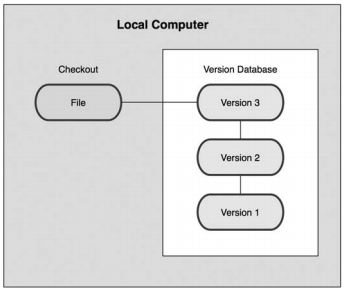
\includegraphics[width=0.4\linewidth]{Bilder/LVKS.png}
%	\captionof{figure}[Lokales Versionssystem Funktionsweise]{Eigene Grafik\footnotemark }
%	\label{fig:osgi}
%\end{minipage}
Natürlich ist diese Variante der Versionskontrolle für Große Projekte die im Team bearbeitet werden eher destruktiv.Ein Beispiel für Lokale Systeme ist RCS( Revision Control System ).Eher geeignet für Teamwork sind die beiden andern Architekturen. 
\subsubsection{Zentralisierte Versionskontrollsysteme}
Bei zentralisierte Versionskontrollsystemen wird die Versionierung nicht lokal vorgenommen. Die Entwickler haben einen Zentralen Punkt, einen Server und dort befindet sich der Quellcode des Projektes in einem Reposytory zu deutsch Lager. Der unterschied zu einfachen Lokalen Systemen ist nun Offensichtlich. Man braucht zumindest ein Netzwerk um solche Systeme zu nutzen. Ein sehr beliebtes zentralisiertes System ist Subversion. Ein weiterer Vorteil gegenüber der lokalen Versionnierung besteht darin das gemeinsames Arbeiten an einem Projekt möglich ist und bei Verwendung eines Servers der Online erreichbar ist kann das Arbeiten auch ohne Ortsbindung ablaufen. Doch dieser Vorteil der Ortsungebundenheit bietet einen enormen „Single Point of Failure“ denn wenn der Server ausfällt ist man nicht in der Lage seiner Arbeit nachzugehen.      

\subsubsection{Verteilte Versionskontrollsysteme}
GIT gehört zu den Verteilten Systemen, der Unterschied zu den Varianten davor ist das sie beides können. 
Einer Art hybride Lösung. Man ist in der Lage Lokal zu Versionieren aber auch im Netzwerk Versionen anderen zur Verfügung zu stellen. Jeder kann als Server fungieren und somit eliminiert man den „Single Point of Failure“ der Zentralisierten Systeme.  

   

\vspace{1em}
\begin{minipage}{\linewidth}
	\centering
	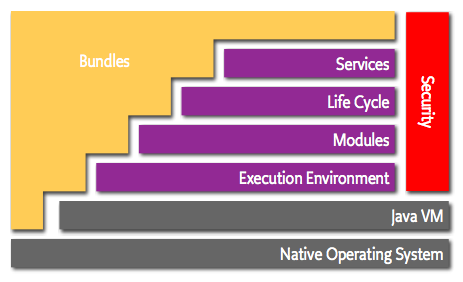
\includegraphics[width=0.7\linewidth]{Bilder/layering-osgi.png}
	\captionof{figure}[OSGi Architektur]{OSGi Architektur\footnotemark }
	\label{fig:osgi}
\end{minipage}
\footnotetext{Quelle: \url{http://www.osgi.org/Technology/WhatIsOSGi}}

\subsection{GIT Historie }
In diesem Abschnitt wird eine Tabelle (siehe Tabelle \ref{tab:beispiel}) dargestellt.

\vspace{1em}
\begin{table}[!h]
	\centering
	\begin{tabular}{|l|l|l|}
		\hline
		\textbf{Name} & \textbf{Name} & \textbf{Name}\\
		\hline
		1 & 2 & 3\\
		\hline
		4 & 5 & 6\\
		\hline
		7 & 8 & 9\\
		\hline
	\end{tabular}
	\caption{Beispieltabelle}
	\label{tab:beispiel}
\end{table}

\pagebreak
\subsection{Anwendungsgebiete von GIT }
Für Auflistungen wird die \textit{compactitem}-Umgebung genutzt, wodurch der Zeilenabstand zwischen den Punkten verringert wird.

\begin{compactitem}
	\item Nur
	\item ein
	\item Beispiel.
\end{compactitem}

\subsection{Listings}
Zuletzt ein Beispiel für ein Listing, in dem Quellcode eingebunden werden kann, siehe Listing \ref{lst:arduino}.

\vspace{1em}
\begin{lstlisting}[caption=Arduino Beispielprogramm, label=lst:arduino]
int ledPin = 13;
void setup() {
    pinMode(ledPin, OUTPUT);
}
void loop() {
    digitalWrite(ledPin, HIGH);
    delay(500);
    digitalWrite(ledPin, LOW);
    delay(500);
}
\end{lstlisting}

\subsection{Tipps}
Die Quellen befinden sich in der Datei \textit{bibo.bib}. Ein Buch- und eine Online-Quelle sind beispielhaft eingefügt. [Vgl. \cite{buch}, \cite{online}]

Abkürzungen lassen sich natürlich auch nutzen (\ac{OSGi}). Weiter oben im Latex-Code findet sich das Verzeichnis.
\pagebreak

% ----------------------------------------------------------------------------------------------------------
% Kapitel
% ----------------------------------------------------------------------------------------------------------
\section{GIT Grundlagen}
Lorem ipsum dolor sit amet.

\subsection{Installation von GIT}
Lorem ipsum dolor sit amet, consetetur sadipscing elitr, sed diam nonumy eirmod tempor invidunt ut labore et dolore magna aliquyam erat, sed diam voluptua. At vero eos et accusam et justo duo dolores et ea rebum. Stet clita kasd gubergren, no sea takimata sanctus est Lorem ipsum dolor sit amet. Lorem ipsum dolor sit amet, consetetur sadipscing elitr, sed diam nonumy eirmod tempor invidunt ut labore et dolore magna aliquyam erat, sed diam voluptua. At vero eos et accusam et justo duo dolores et ea rebum. Stet clita kasd gubergren, no sea takimata sanctus est Lorem ipsum dolor sit amet.

\subsection{Konfiguration von GIT}
Lorem ipsum dolor sit amet, consetetur sadipscing elitr, sed diam nonumy eirmod tempor invidunt ut labore et dolore magna aliquyam erat, sed diam voluptua. At vero eos et accusam et justo duo dolores et ea rebum. Stet clita kasd gubergren, no sea takimata sanctus est Lorem ipsum dolor sit amet. Lorem ipsum dolor sit amet, consetetur sadipscing elitr, sed diam nonumy eirmod tempor invidunt ut labore et dolore magna aliquyam erat, sed diam voluptua. At vero eos et accusam et justo duo dolores et ea rebum. Stet clita kasd gubergren, no sea takimata sanctus est Lorem ipsum dolor sit amet.

\subsection{Hilfestellungen durch das System}
Lorem ipsum dolor sit amet, consetetur sadipscing elitr, sed diam nonumy eirmod tempor invidunt ut labore et dolore magna aliquyam erat, sed diam voluptua. At vero eos et accusam et justo duo dolores et ea rebum. Stet clita kasd gubergren, no sea takimata sanctus est Lorem ipsum dolor sit amet. Lorem ipsum dolor sit amet, consetetur sadipscing elitr, sed diam nonumy eirmod tempor invidunt ut labore et dolore magna aliquyam erat, sed diam voluptua. At vero eos et accusam et justo duo dolores et ea rebum. Stet clita kasd gubergren, no sea takimata sanctus est Lorem ipsum dolor sit amet.
\pagebreak

% ----------------------------------------------------------------------------------------------------------
% Kapitel 
% ----------------------------------------------------------------------------------------------------------
\section{KAp}
Lorem ipsum dolor sit amet.

\subsection{Unterkapitel}
Lorem ipsum dolor sit amet, consetetur sadipscing elitr, sed diam nonumy eirmod tempor invidunt ut labore et dolore magna aliquyam erat, sed diam voluptua. At vero eos et accusam et justo duo dolores et ea rebum. Stet clita kasd gubergren, no sea takimata sanctus est Lorem ipsum dolor sit amet. Lorem ipsum dolor sit amet, consetetur sadipscing elitr, sed diam nonumy eirmod tempor invidunt ut labore et dolore magna aliquyam erat, sed diam voluptua. At vero eos et accusam et justo duo dolores et ea rebum. Stet clita kasd gubergren, no sea takimata sanctus est Lorem ipsum dolor sit amet.

\subsection{Unterkapitel}
Lorem ipsum dolor sit amet, consetetur sadipscing elitr, sed diam nonumy eirmod tempor invidunt ut labore et dolore magna aliquyam erat, sed diam voluptua. At vero eos et accusam et justo duo dolores et ea rebum. Stet clita kasd gubergren, no sea takimata sanctus est Lorem ipsum dolor sit amet. Lorem ipsum dolor sit amet, consetetur sadipscing elitr, sed diam nonumy eirmod tempor invidunt ut labore et dolore magna aliquyam erat, sed diam voluptua. At vero eos et accusam et justo duo dolores et ea rebum. Stet clita kasd gubergren, no sea takimata sanctus est Lorem ipsum dolor sit amet.
\pagebreak

% ----------------------------------------------------------------------------------------------------------
% Kapitel
% ----------------------------------------------------------------------------------------------------------
\section{Kapitel}
Lorem ipsum dolor sit amet.

\subsection{Unterkapitel}
Lorem ipsum dolor sit amet, consetetur sadipscing elitr, sed diam nonumy eirmod tempor invidunt ut labore et dolore magna aliquyam erat, sed diam voluptua. At vero eos et accusam et justo duo dolores et ea rebum. Stet clita kasd gubergren, no sea takimata sanctus est Lorem ipsum dolor sit amet. Lorem ipsum dolor sit amet, consetetur sadipscing elitr, sed diam nonumy eirmod tempor invidunt ut labore et dolore magna aliquyam erat, sed diam voluptua. At vero eos et accusam et justo duo dolores et ea rebum. Stet clita kasd gubergren, no sea takimata sanctus est Lorem ipsum dolor sit amet.

\subsection{Unterkapitel}
Lorem ipsum dolor sit amet, consetetur sadipscing elitr, sed diam nonumy eirmod tempor invidunt ut labore et dolore magna aliquyam erat, sed diam voluptua. At vero eos et accusam et justo duo dolores et ea rebum. Stet clita kasd gubergren, no sea takimata sanctus est Lorem ipsum dolor sit amet. Lorem ipsum dolor sit amet, consetetur sadipscing elitr, sed diam nonumy eirmod tempor invidunt ut labore et dolore magna aliquyam erat, sed diam voluptua. At vero eos et accusam et justo duo dolores et ea rebum. Stet clita kasd gubergren, no sea takimata sanctus est Lorem ipsum dolor sit amet.
\pagebreak

% ----------------------------------------------------------------------------------------------------------
% Literatur
% ----------------------------------------------------------------------------------------------------------
\renewcommand\refname{Quellenverzeichnis}
\bibliographystyle{myalpha}
\bibliography{bibo}
\pagebreak

% ----------------------------------------------------------------------------------------------------------
% Anhang
% ----------------------------------------------------------------------------------------------------------
\pagenumbering{Roman}
\setcounter{page}{1}
\lhead{Anhang \thesection}

\begin{appendix}
\section*{Anhang}
\phantomsection
\addcontentsline{toc}{section}{Anhang}
\addtocontents{toc}{\vspace{-0.5em}}

\section{GUI}
Ein toller Anhang.

\subsection*{Screenshot}
\label{app:screenshot}
Unterkategorie, die nicht im Inhaltsverzeichnis auftaucht.

\end{appendix}


\newpage
\thispagestyle{empty}
\begin{center}
	\vspace*{5em}
	\huge\textbf{Erklärung}\\
\end{center}
\vspace{2em}
Hiermit versichere ich, dass ich meine Abschlussarbeit selbständig verfasst und keine anderen als die angegebenen Quellen und Hilfsmittel benutzt habe.

\vspace{4em}
\begin{minipage}{\linewidth}
	\begin{tabular}{p{15em}p{15em}}
		Datum: &  .......................................................\\
		& \centering (Unterschrift)\\
	\end{tabular}
\end{minipage}

\end{document}
